Athena uses a number of unit tests during the development lifecycle to ensure core I/O functionality does not break.
Many of the I/O tests were originally created for the old EDM and haven't been updated to test the xAOD EDMs core I/O functions.
This project took in track information from a unit test using the T/P EDM, writes the data into an example xAOD object to file and reads it back.


\section{xAOD Test Object}
\label{sec:Mod_utests_xAOD_object}

% Overview
The object used to employ the new unit test is the \verb|xAOD::ExampleElectron| object, where the \verb|xAOD::| is a declaration of the namespace and simply identifies the object as an xAOD object.
An individual \verb|ExampleElectron| object only has a few parameters for sake of testing, its transvese momentum, \verb|pt|, and its charge, \verb|charge|.
A collection of \verb|ExampleElectron| objects are stored in the \verb|ExampleElectronContainer| object, which is just a \verb|DataVector| of \verb|ExampleElectron| objects.\cite{Buckley_2015}
This \verb|DataVector<xAOD::ExampleElectron>| acts similar to a \verb|std::vector<xAOD::ExampleElectron>|, but has additional code to handle the separation of interface and auxiliary data storage. 

% Aux Store
The xAOD EDM uses an abstract interface connecting between the \verb|DataVector| and the auxiliary data, this is the \verb|IAuxStore|. 
The function \verb|setStore| is responsible for ensuring the auxillary data store is matched with it's corresponding \verb|DataVector|.
Another feature to the xAOD EDM is the ability to have a dynamic store of auxiliary data.
This separates the auxiliary data between static and dynamic data stores. 
Where the static dta stores comprise of known variables and the dynamic counterpart stores data of variables not declared but still might be needed by the user. 
Figure \ref{fig:Mod_utests_aux_store} illustrates how a simple setup of storing a \verb|DataVector| of electrons that hold some specific parameters into one \verb|IAuxStore| while also having a separate \verb|IAuxStore| specifically for the dynamic attributes. 

\begin{figure}[h]
    \centering
    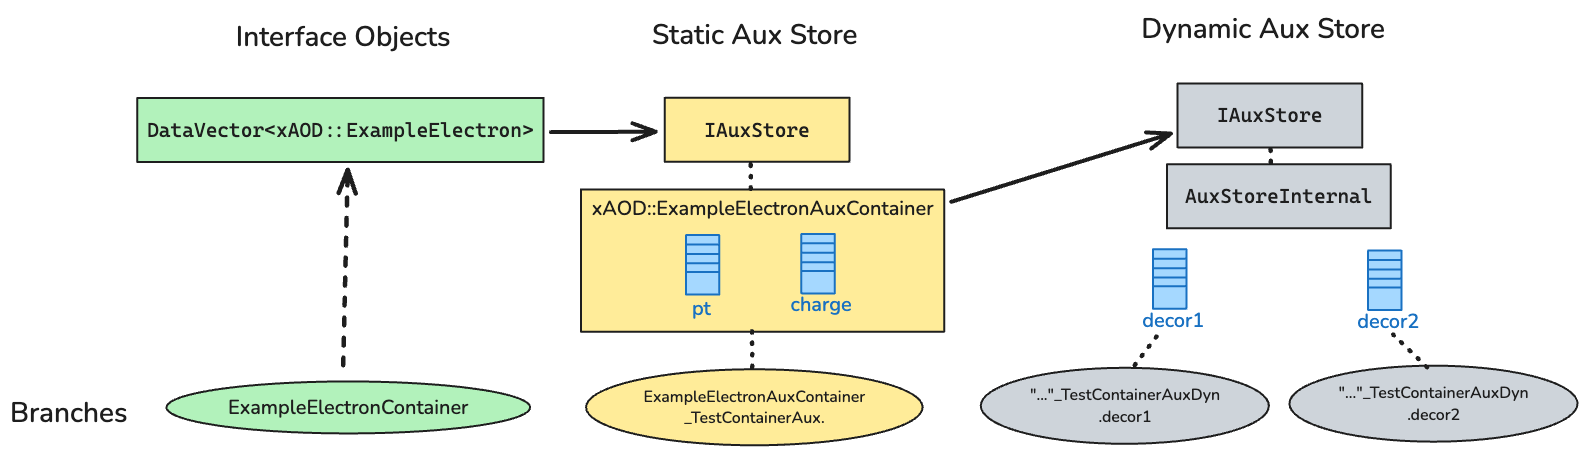
\includegraphics[width=\textwidth]{content/img/aux_store_better.png}
    \caption{The static and dynamic auxiliary data store for a collection of xAOD::ExampleElectrons.}
    \label{fig:Mod_utests_aux_store}
\end{figure}





\section{Unit Tests}
\label{sec:Mod_utests_CI}
Unit tests are programs that act as a catch during the continuous integration of a codebase and exhaust features that need to remain functional. 
Athena has a number of unit tests which check every merge request and nightly build for issues in the new code that could break core functionality, either at the level of Athena, ROOT, or any other software in the LCG stack.
With the adoption of the xAOD EDM, there were no unit tests to cover core I/O functionality related to this new EDM. 

Specifically there were no unit tests to handle selection of dynamic attributes, or decorations, on xAOD objects created during writing and read back.
To address this, a new xAOD test object needed to be created and written during a new unit test that fit into the existing unit tests.
The list of AthenaPoolExample unit tests that are currently executed during a nightly build can be found in Table \ref{tab:CI_Unit_Tests}.
These tests are executed in this order, as the objects created in one might be used in proceeding test.

\begin{table}[h]
    \centering
    % \resizebox{\textwidth}{!}{
    \begin{tabular}{|c|c|}
        \hline
        $\textbf{Unit Test}$ & $\textbf{Employed Algorithms}$ \\
        \hline
        Write & WriteData \\
        \hline
        ReadWrite & ReadData \\
        \hline
        Read & ReadData \\
        \hline
        Copy & None \\
        \hline
        ReadWriteNext & ReadData, ReWriteData \\
        \hline
        WritexAODElectron & ReadData, WriteExampleElectron \\
        \hline
        ReadxAODElectron & ReadExampleElectron \\
        \hline
        ReadAgain & ReadData \\
        \hline
        WriteConcat & WriteData, ReWriteData \\
        \hline
        ReadConcat & ReadData \\
        \hline
        WriteCond & ReadData, WriteCond \\
        \hline
        ReadCond & ReadData, ReadCond \\
        \hline
        WriteMeta & WriteData, WriteCond \\
        \hline
        ReadMeta & ReadData \\
        \hline
    \end{tabular}
    % }
    \caption{List of unit tests in the AthenaPoolExample package that are currently executed during a nightly build.}
    \label{tab:CI_Unit_Tests}
\end{table}

The mechanism for passing a unit test is done automatically by building the framework, running the unit tests, and comparing the diff of the output file to the unit test with a reference file associated with that particular unit test. 
If the unit test passes, then the diff will be empty and the unit test will be marked as passing.
Conversely, if the unit test fails, then the diff will be non-empty and the unit test will be marked as failing.

\subsection{WritexAODElectron.py}
The two new tests were \verb|WritexAODElectron| and \verb|ReadxAODElectron|.
During the \verb|WritexAODElectron| unit test, the first call is to the \verb|ReadData| algorithm to read off all of the \verb|ExampleTrack| objects stored in one of the files produced by the \verb|ReadWrite| unit-test.
Then the \verb|WriteExampleElectron| algorithm is called and takes \verb|ExampleTracks|, creates an \verb|ExampleElectron| object and sets the electrons \verb|pt| to the tracks \verb|pt|. 

\begin{figure}[h]
    \centering
    \begin{lstlisting}[language=C]
        auto elecCont = std::make_unique<xAOD::ExampleElectronContainer>();
        auto elecStore = std::make_unique<xAOD::ExampleElectronAuxContainer>();
        elecCont->setStore(elecStore.get());

        SG::ReadHandle<ExampleTrackContainer> trackCont(m_exampleTrackKey, ctx);
    
        elecCont->push_back(std::make_unique<xAOD::ExampleElectron>());
      
        for (const ExampleTrack* track : *trackCont) {
          // Take on the pT of the track
          elecCont->back()->setPt(track->getPT());
        }

        SG::WriteHandle<xAOD::ExampleElectronContainer> objs(m_exampleElectronContainerKey, ctx);
        ATH_CHECK(objs.record(std::move(elecCont), std::move(elecStore)));
    \end{lstlisting}
    \label{fig:Mod_utests_WritexAODElectron1}
\end{figure}
As shown in Figure \ref{fig:Mod_utests_WritexAODElectron1}, the \verb|ExampleElectronContainer| and \verb|ExampleElectronAuxContainer| are created and set to the \verb|elecCont| and \verb|elecStore| respectively.
The \verb|elecCont| has an associated aux store, so the \verb|setStore| function is called with the \verb|elecStore| pointer.
The track container is accessed by using StoreGate's \verb|ReadHandle|, which associates the \verb|m_exampleTrackKey| with the \verb|ExampleTrackContainer| specified in the header file.
This is then looped over all elements in the container and the \verb|pt| of each track is set to the \verb|pt| of the electron.
A \verb|WriteHandle|, called \verb|objs|, is then created for the container of \verb|ExampleElectrons| which is then recorded.

Within the same algorithm, the next step is to loop over each of the newly produced \verb|ExampleElectrons|, accessing the decorations \verb|decor1| and \verb|decor2|, and setting each to an arbitrary float value that are easily identifiable later.
Figure \ref{fig:Mod_utests_WritexAODElectron2} shows how this is done using two handles for each decoration. 
Note the difference here using the \verb|WriteDecorHandle|, where the prior handle type was \verb|WriteHandle|.
\begin{figure}[h]
    \centering
    \begin{lstlisting}[language=C]
        SG::WriteDecorHandle<xAOD::ExampleElectronContainer, float> hdl1(m_decor1Key,ctx);
        SG::WriteDecorHandle<xAOD::ExampleElectronContainer, float> hdl2(m_decor2Key,ctx);

        for (const xAOD::ExampleElectron* obj : *objs) {
            hdl1(objs) = 123.;
            hdl2(objs) = 456.;
        }
    \end{lstlisting}
    \label{fig:Mod_utests_WritexAODElectron2}
\end{figure}


\subsection{ReadxAODElectron.py}
The \verb|ReadxAODElectron| unit test will attempt to show the xAOD function of accessing one dynamic variable, in this case \verb|decor1|, while not accessing the other, \verb|decor2|.


\section{Results}
